
\section*{Exercise 2}
\label{sec:exercise-2}

\subsection*{(a)}
\label{sec:a-1}

The scatter plot can be found in Figure \ref{fig:ex2-scatter} the outlier can be
clearly be seen at $x_1 = 284$.
\begin{figure}[h]
  \centering
  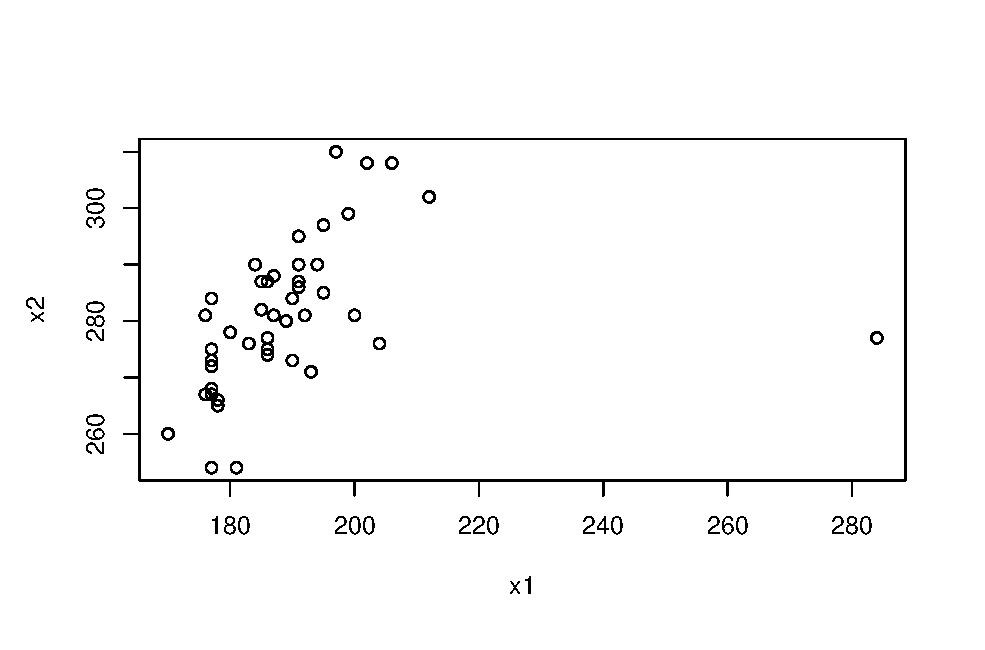
\includegraphics[width=5cm]{ex2-scatterplot}
  \caption{Scatter plot of the tail length and the wing span for male
    hook-billed kites.}
  \label{fig:ex2-scatter}
\end{figure}

\subsection*{(b)}
\label{sec:b-1}

Using the Box corrected test found in \cite[p. 311]{book}, we find that
we can not pool the covariance matrices (see code for details).

\subsection*{(c)}
\label{sec:c-1}

In this test, the pooled matrix $S_p$ was used. Using the Hotelling's
$T^2$ test, we can put $\delta = \bar{x}_{\rm male}- \bar{x}_{\rm
  female}$, we can use the test variable
\begin{equation*}
  T^2 = \frac{n_{\rm female}  n_{\rm male}}{n_{\rm female} +  n_{\rm male}}\delta^T S_p^{-1}\delta,
  \label{eq:1}
\end{equation*}
and rejected $H_0: \mu_{\rm male} = \mu_{\rm female}$ if the test
variable is larger than
\begin{equation*}
 c  = \frac{fp}{f-p+1}F_{1-\alpha}(p, n-p), %c = f*p*qf(1-0.05, p, f-p)/(f-p+1)
\end{equation*}
where $f = n - 1$, and $p = 2$. Since $T^2 = 7.494772$ and $c =
6.27986$, we reject $H_0: \mu_{\rm male} = \mu_{\rm female} $.

The result would most likely hold if we changed the value of the
outlier to $x_1 = 184$ instead of 284, since the sample size should be too
large enough for any drastic changes in the variance matrix or mean to
happen.

\subsection*{(d)}
\label{sec:d}
??

\subsection*{(e)}
\label{sec:e}

The confidence region if given by the equation, for $\mu = (\mu_1, \mu_2).$
\begin{equation}
  \label{eq:ex2-conf-region}
 \{\mu:\ n (\delta - \mu)^T S_p^{-1} (\delta-\mu)\leq \frac{(n-1)p}{n-p}F_{1-\alpha}(p,n-p)\},
\end{equation}
where $\alpha = 0.05$, $S_p$ is the pooled matrix from the previous
exercise, and $\delta = \bar{x}_{\rm male}  - \bar{x}_{\rm
  female}$. Computing the LHS of \eqref{eq:ex2-conf-region}, get
\begin{align*}
  89
  \big(
    &206.7294 ( - 6.463131 -\mu_1)^2 + 189.1233(1.176768 -\mu_2)^2 \\
    &+ 202.2905(- 6.463131 - \mu_1)(1.176768- \mu_2)
  \big)\\
  &\leq \frac{88\cdot 2}{87}3.103839
\end{align*}
Further, to find the confidence intervals for the the different
components, we use the vectors $a_1 = (1,0)^T$ and $a_2 = (0,1)^T$, to
create each of the component wise intervals, respectively. The
intervals, for each $a$, is given by 
\begin{equation*}
  n_f n_m \delta^T S_p^{-1} \delta / (n_f + n_m) , 
\end{equation*}
where.
we get the intervals
\begin{align*}
  (-170.698117786475&; 157.771855160212), \quad \text{for } a = (1,0)
  \\
  (-149.071120157853&;151.424655511388), \quad \text{for } a = (0,1)
\end{align*}

\subsection*{(f)}
\label{sec:f}

From the interval we find the Exercise (e), we see that there are no
genrall difference for the lengths between the female and the male birds.
\subsection*{\texttt{R} code}
\label{sec:textttr-code}

\lstinputlisting[style=R]{../ex2.R}

%%% Local Variables:
%%% mode: latex
%%% TeX-master: "examination"
%%% End:
